\documentclass[letterpaper, 12 pt, conference]{ieeeconf}  % Comment this line out if you need a4paper

\IEEEoverridecommandlockouts                        
\overrideIEEEmargins                                      % Needed to meet printer requirements.

\usepackage{booktabs}
\usepackage{graphicx}
\usepackage{cite}
\usepackage{url}
\usepackage{algorithm}
\usepackage{algorithmic}
\usepackage{amsmath}
\usepackage{caption}
\usepackage{subcaption}
\usepackage{units}
\usepackage{wrapfig} % Wraps text round images
\usepackage{epstopdf}
\usepackage{amsmath}
\usepackage{listings}    
\usepackage{hyperref}
\usepackage{acronym}
\usepackage{multicol}


\acrodef{KT}{Kinesio Tape}
\acrodef{ROI}{region of interest}
\acrodef{KRS}{Department of Kinesiology and Rehabilitation Science}
\acrodef{ABP}{Department of Anatomy, Biochemistry \& Physiology}
\acrodef{HDRS}{Hawaii Diagnostic Radiography Services}


\newtheorem{definition}{Definition} 

\DeclareMathOperator{\diff}{diff}
\DeclareMathOperator{\adv}{adv}
\DeclareMathOperator{\card}{card}



\title{\LARGE  Quantitative analysis of the effects of Kinesio Tape}%
\author{by Nathaniel Saul \\ Advisor: Dr. Yuriy Mileyko} 

\begin{document}





\section{Introduction}
\subsection{Description of tape}
used by athletes.  in the olympics.  very stretchy, sticks on, and stays for a few days. people say it helps with injury recovery, injury prevention, and performance.
\subsection{outline of previous research on the tape}
meta studies, subjective studies.  mostly testimonial,  "32 people say it helps them" is a marketing scheme, not a science.
\subsection{Hypothesis}
That the claimed cause could is a result of the expansion of the subcutaneous region, but many others claim that it is just placebo and doesn't really do anything.  There hasn't been any objective look at the effects of the tape, and so it is still legal for use.  

\section{Problem statement}
\subsection{Null Hypothesis}
The null hypothesis is that there is no significant change
\subsection{Make it easy for nonmathematicians.}
  Also, explore ways to quantify complex data in meaningful ways for people who don't know about complex data.
we have to distill the change in shape down to just a handful of simple, understandable numbers or images.

we should walk away with a general purpose method for analyzing this kinds of shape change of any arbitrary shape.


using extremely complex methods is useless if we are unable to present the results of those methods in a meaningful way.   need a nice picture that sums up the change and a nice number that sums up the change -- p-values are great numbers for this purpose.  

\section{Description of data format}

Researchers at the Kinesiology department and JABSOM are collecting MRI of athletes before and during application of the tape.
(now that they have the IRB review!!)
\subsection{8 landmarks on thigh and triangulation in between}
4 spots (of some chemical) that shows up on the mri scanners, then lines are drawn radially inwards until they hit muscle and this defines the region of interest (ROI). 
\subsection{very noisy... topological issues. handles make the data unusable to the algorithms - assume topologically equivalent to disk}
The region is then extracted.  They focus on the density to isolate the different regions, see Figure~\ref{fig:thigh_slice} 

images of the not cleaned up thigh..  emphasis different connected components and the topological features.  
\subsection{triangulations from MRI .}
- no central axis - each person is different size and laying differently through out.  we use general procrustes method to align and resize all the shapes - iterative algorithm
show a picture of simple images being aligned



\section{Landmark based methods}
\subsection{Hotelling's t-test. }
pretty straight forward analysis

 a multidimensional generalization of the t-test.  tests whether or not the means of points are different
 
compares the differences in positions of each point over time for each person. 8 points, 3 time steps, that is 24 differences.  so we can test how likely it is that this mean is zero.


assuming the corners play a large role in the shape change...




\section{entire ROI based methods}

what if the corners don't change much?  There is a whole bunch of information that is lost - like (n-8)/n \% vertices and edges worth of data that is lost.  what if the shape wrinkles a little bit, only in the center, or if 

\subsection{parameterize the surface}
map each surface to the unit cube:  

take the landmarks, find the nearest neighboring vertex using the nearest neighbor search.  Then find the shortest paths between these vertices using the Dijkstra's shortest path algorithm.  Along these paths, cut out the 6 sides of the shape.  Each of these 6 sides, map to the unit square.  Using the Mean Floater algorithm. 

\subsection{do statistics on the parameterized surface}

then we can compare these shapes in an ordered way.  by saying, look at each point on the unit square, and see how the correlated point on each shape is different from each other.  

for this shape, a method that we are implementing will compare the distances between the corresponding top and bottom points.  Then for the mean shape, we can create a map of p-values describing whether the change at that point across all the patients was significant.  This is easy to look at and see which part of the image changed the most (or is most likely to change at all).  we 

\subsection{work is still continuing}
ways of computing persistence diagrams of each parameterized image. then we can compute statistics on the persistence diagrams.



\section{challenges/reflections/next steps}
\subsection{challenges}
working with these very complex libraries for graph and triangulation algorithms was hard.  Hardest part was trying to do all this development with only assumptions of what the images were going to look like.  trrying to design a black box method in which the input was ill defined is really hard and obnoxious because it forces you to make all sorts of assumptions that impact the design.  it is reassuring to know what the data looks like so you don't have to assume so much.  
\subsection{next steps}
the images still have not shown up, and it's not completely finished.  So we will continue to develop methods.  currently trying to get the corners set... and... 





\begin{figure}[h!]
  \caption{thigh cross section with density information}
  \centering
    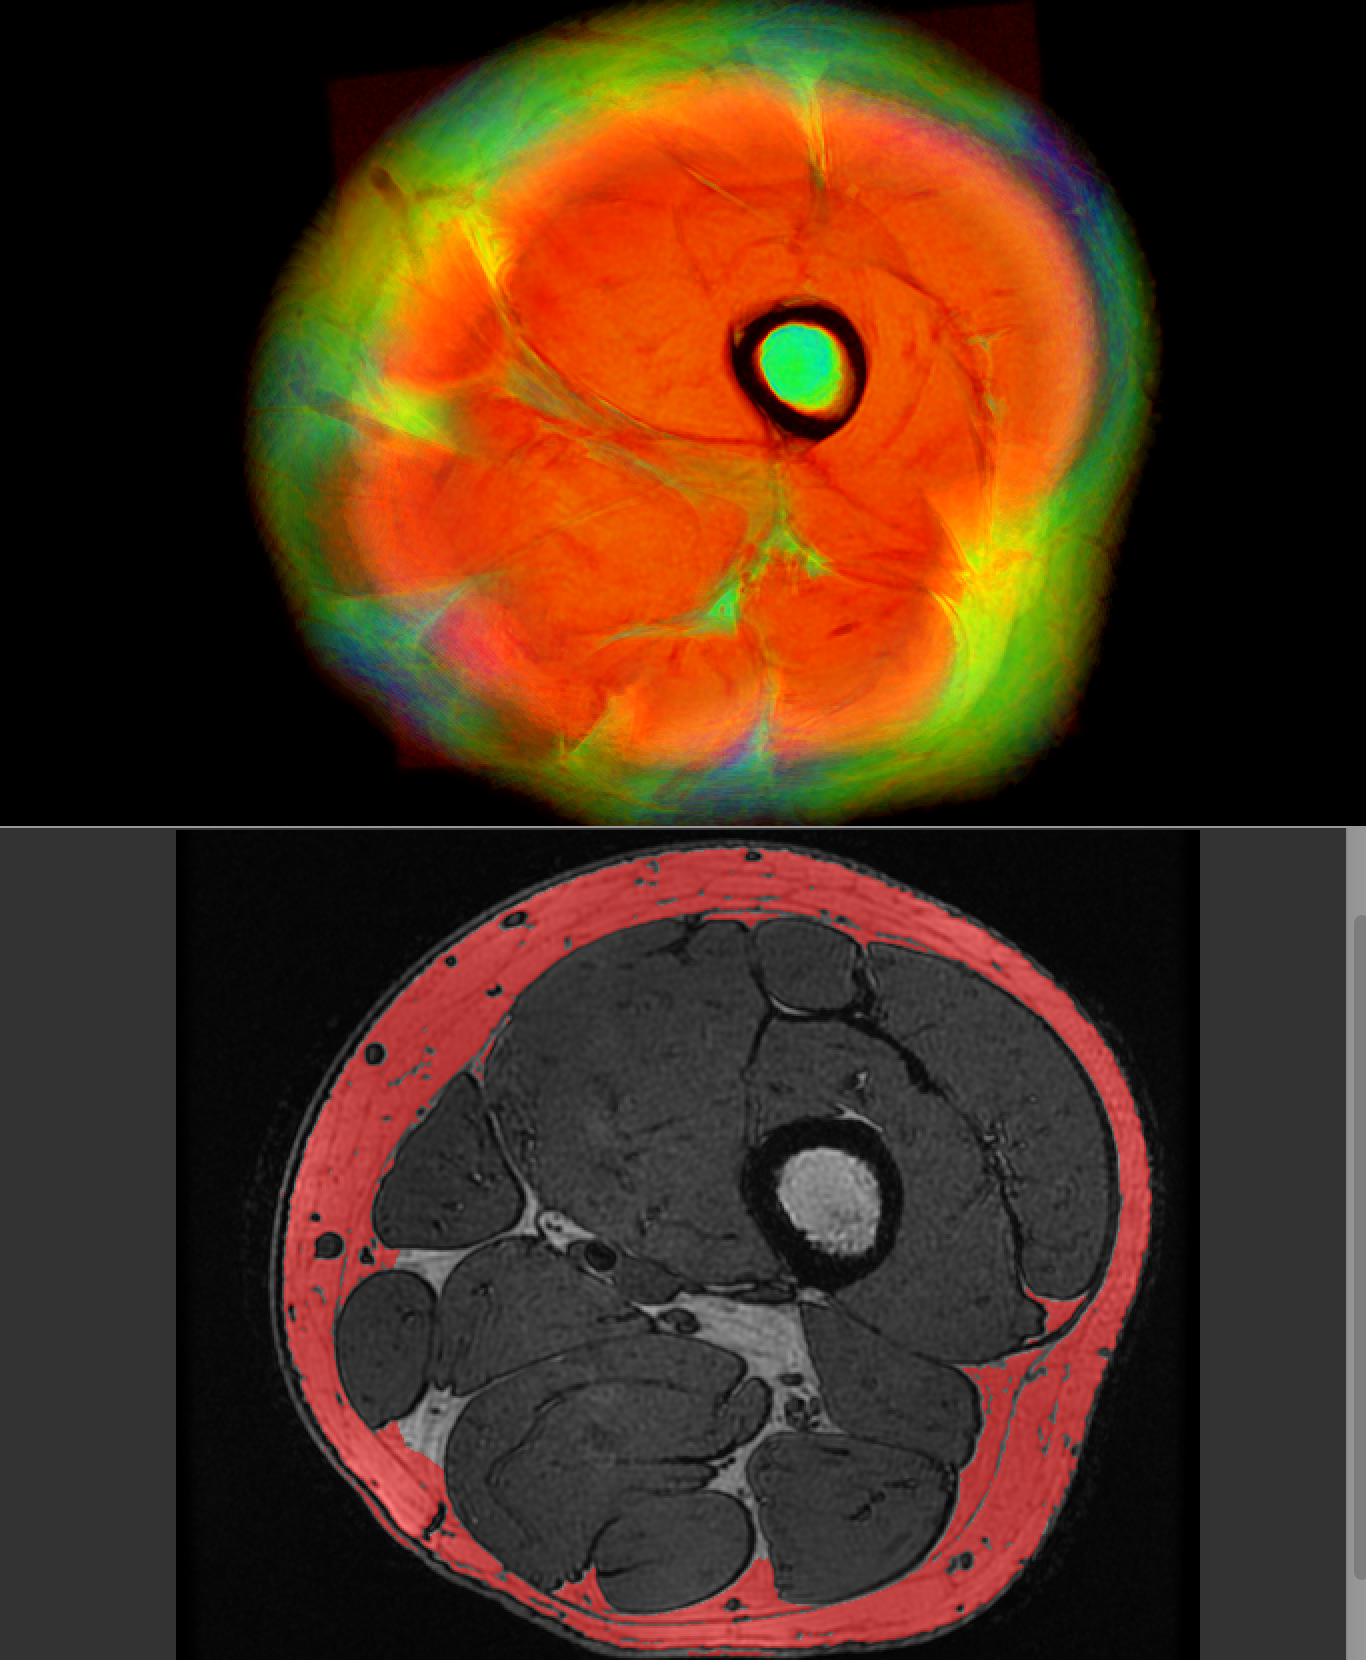
\includegraphics[width=0.5\textwidth]{images/thigh_slice.png}
    
      \label{fig:thigh_slice}

\end{figure}


\begin{figure}[h!]
  \caption{thigh with highlighted region of interest.}
  \centering
    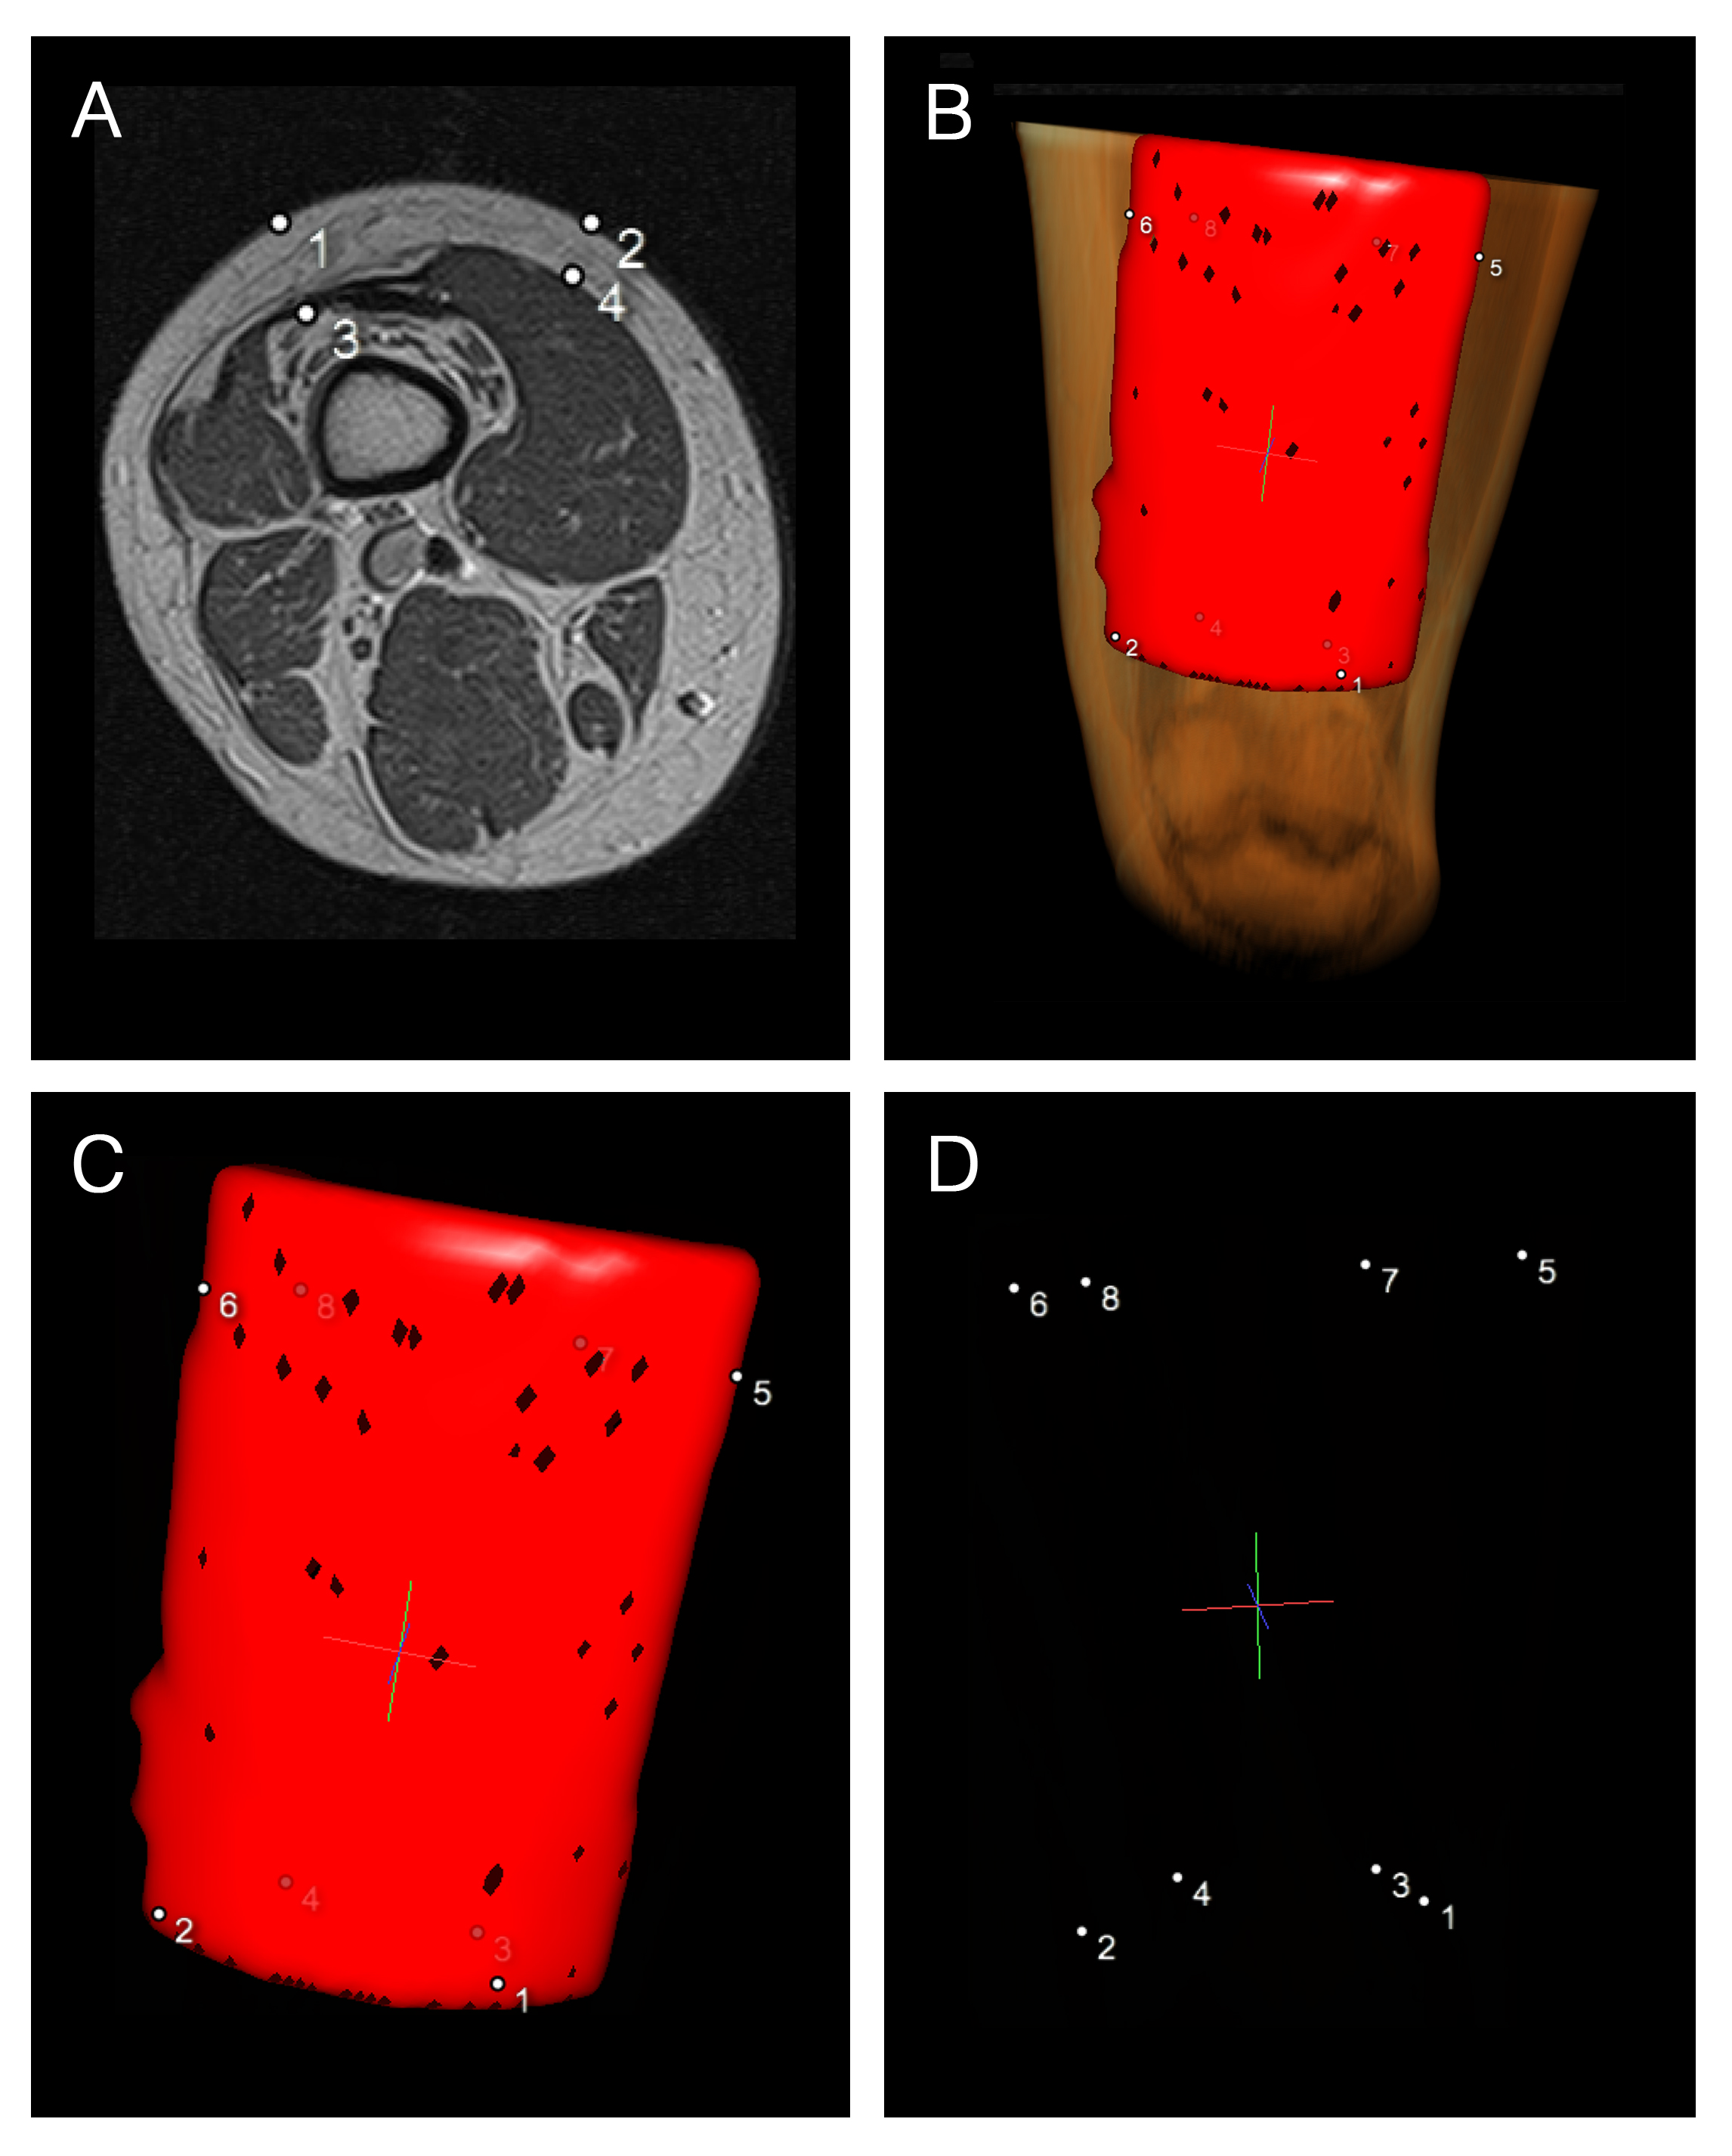
\includegraphics[width=0.5\textwidth]{images/thighwROI.jpg}
    
    \label{fig:thighwROI}
\end{figure}

\begin{figure}[h!]
  \caption{scross sections of thighl.}
  \centering
    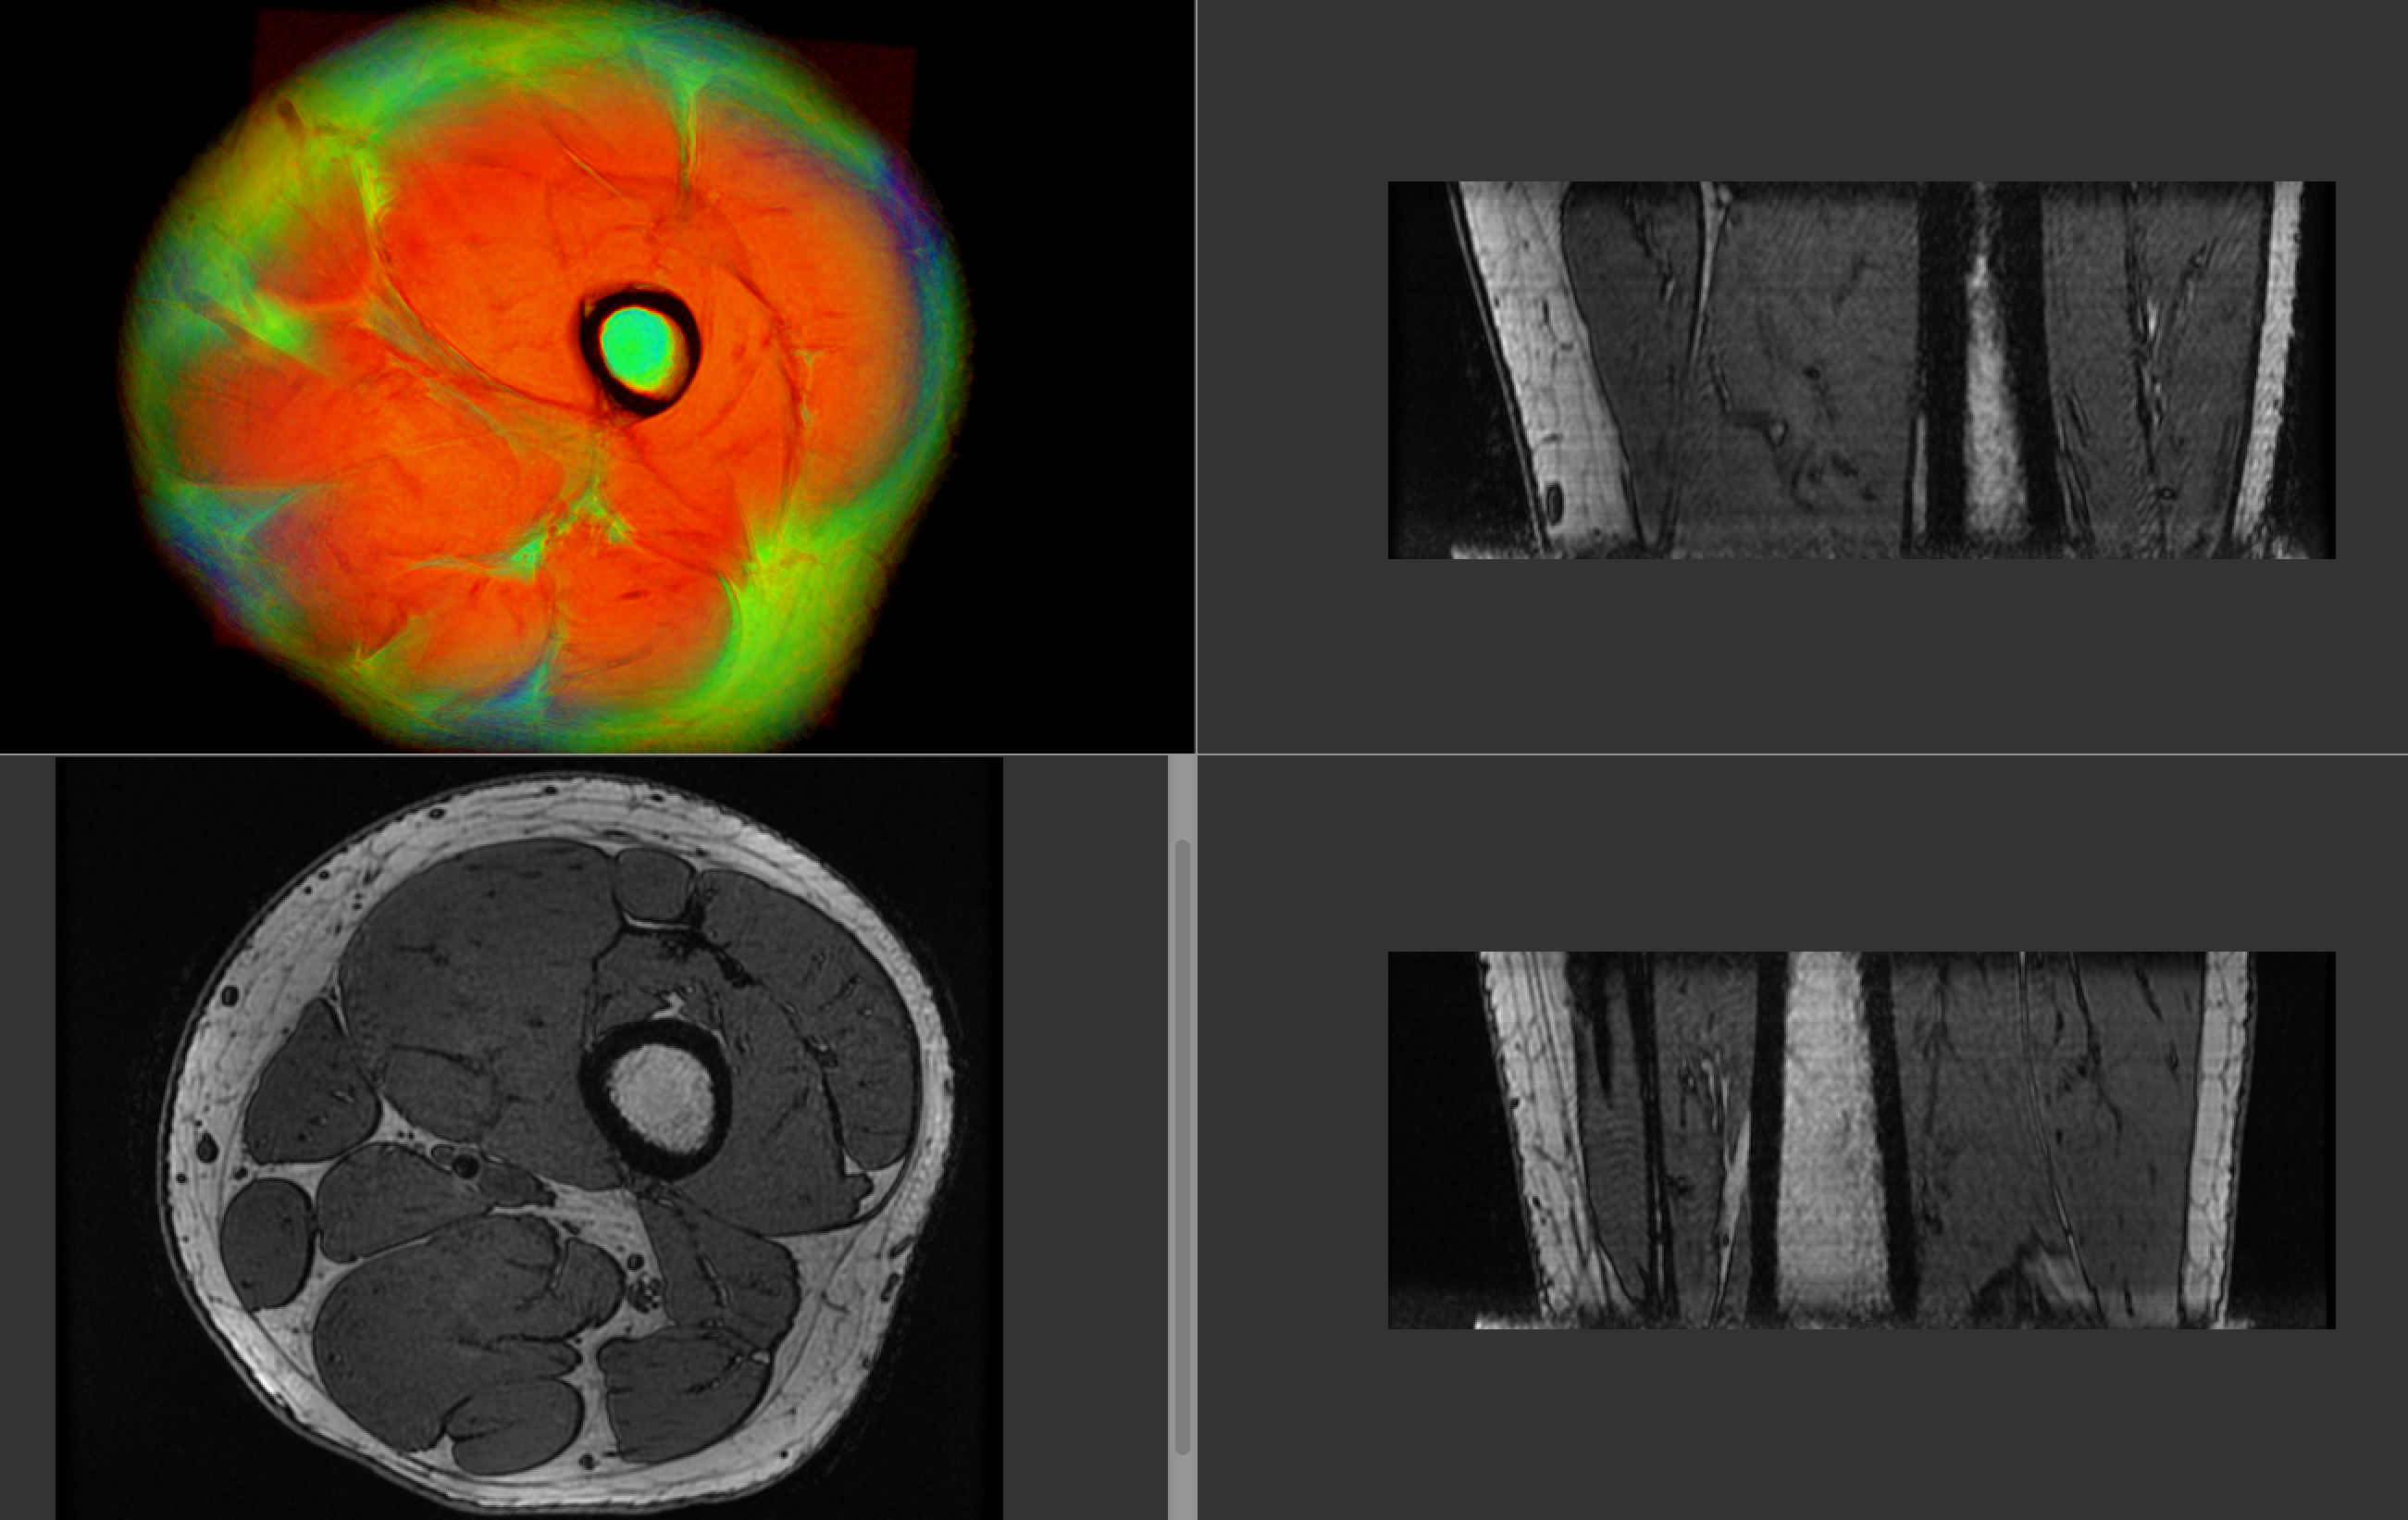
\includegraphics[width=0.5\textwidth]{images/thigh_colored.png}
    \label{fig:thigh_colored}
\end{figure}

\begin{figure}[h!]
  \caption{extracted region of interest.}
  \centering
    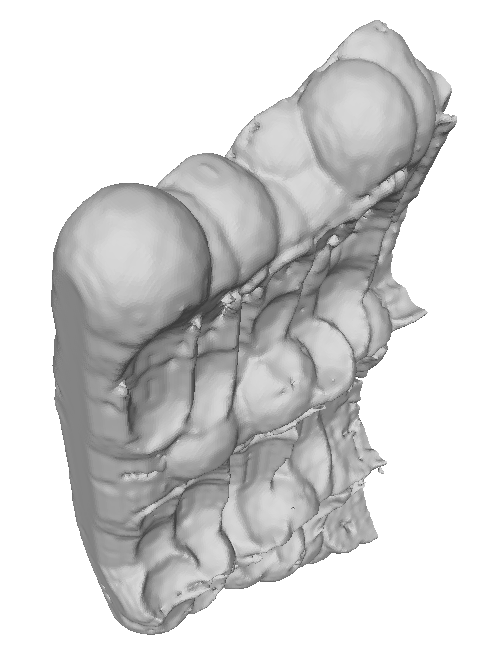
\includegraphics[width=0.5\textwidth]{images/snapshot_angled02.png}
    \label{fig:angled}
\end{figure}

\begin{figure}[h!]
  \caption{highlight of topological impurities.}
  \centering
    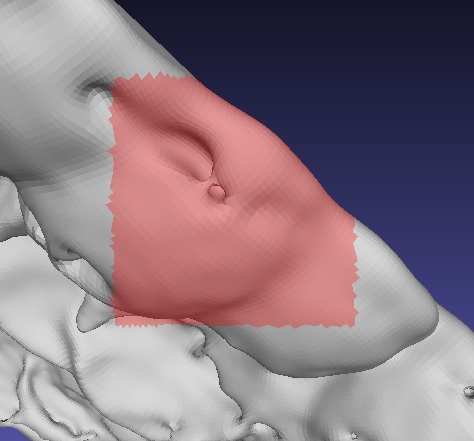
\includegraphics[width=0.5\textwidth]{images/loop_example.jpg}
    \label{fig:loop}
\end{figure}

\maketitle
\thispagestyle{empty}
\pagestyle{empty}

















































\section{Inquiry Statement}  

 \ac{KT} is made from elastic cotton designed to stretch up to 40\% its static length. When the tape is applied to the skin it recoils and pulls on the surface. It is highly breathable and can be kept on for upwards of four days. \ac{KT} gained popularity following the 2008 Olympics in Beijing and is now commonly used by athletes at all levels of training and competition.   Manufacturers claim that applications of the tape can decrease pain from injuries, prevent injuries, and provide increased performance of the muscles directly below the tape.     

These claimed benefits could be a result of the tape exerting a pressure that expands the space deep under the skin.  This expansion would potentially restore epidermal tissue homeostasis while increasing fluid movement, diminish pain by decreasing pressure on associated receptors, and possibly facilitate improved tensile properties of the deep fascia enveloping muscles. A few short-term studies have been conducted that addressed the subjective responses of test subjects using \ac{KT} \cite{Konishi2013}\cite{Osorio2013} \cite{OSullivan2011} but currently, no studies have been conducted concerning the underlying mechanism and functional effects of the \ac{KT}.

A collaborative effort including expertise from the Department of Mathematics, \ac{ABP}, \ac{KRS}, and the \ac{HDRS} at St. Francis Hospital has been organized to address this lack of experimental evidence. We hypothesize that the form of the subcutaneous compartment of the thigh is altered as a result of KT application in human subjects. To test this hypothesis, the research team will analyze MR images of the area affected by the tape. 

Currently, there are no well-defined methods for quantitatively analyzing the effects of the \ac{KT}.  This project focuses on an important subcomponent of the larger collaborative research project: to research, evaluate, and apply novel analysis methods to identification and quantification of changes resulting from \ac{KT} use.  

The project aims to develop a novel approach to analysing the region affected by \ac{KT} and to implement the approach in a software application.  This software will quantify the change of size and/or shape of the subcutaneous compartment of an individual and compare changes between individuals over the course of the study.


This project will, in the first instance, provide a quantitative approach that specifically determines whether KT repositions the subcutaneous compartment in a fashion that could improve fluid dynamics improving an athlete's performance.  However, this study is expected to provide a more general solution for quantitative assessment of morphological changes derived from advanced medical images such as MR, CT, spiral CT, etc, that could ultimately have broad implications for diagnostic and therapeutic outcomes beyond the current project.  





%%%%%%%%%%%%%%%%%%%%%%%%%%%%%%%
\section{Objectives/Methods}

Over the next three months, researchers at \ac{KRS} and St. Francis will collect time-series MR images of students using the tape.  Next, under guidance from Dr. Mileyko, I will develop novel methods to analyze these images and implement them in a computer application.  Finally, Dr. Lozanoff from the \ac{ABP} and I will use this new tool to analyze the MR images and draw conclusions about the effects of \ac{KT}.

\subsection{Image Collection}

Researchers at \ac{KRS} and \ac{HDRS} will collect MR images of 20 participants with iliotibial band syndrome and 20 healthy participants for this study.  A customized length of \ac{KT} will be applied to the thigh with 15\% tension according to the Kinesio EDF Taping Manual. Small oil beads will be placed at standardized areas of the thigh to provide reference points on the MR images.  Subjects will be scanned at time 0 ($T_0$), 24 hours ($T_1$) and 48 hours ($T_2$) following placement of the tape. Once scanning is completed, additional landmarks will be identified and the desired region for analysis will be segmented. This aspect of the project is currently under IRB review.

\subsection{Shape Analysis Methods}

The next portion of the project will be the entire focus of this proposal.  It will involve the development the shape analysis methods and their implementation in a software application.   The software will test whether there is a shape and/or size change in the \ac{ROI} and quantify this change in a meaningful way.  Additionally, it will quantify the change in \ac{ROI} for an individual (intra-personal) and between individuals (inter-personal) over time.  

We will complete this in three steps.  First, Dr. Mileyko and I will complete a literature review of current methods.  We will then choose which methods could be particularly promising and potentially design new methods based on some of Dr. Mileyko's past work.  Finally, we will implement the methods in a software application and test their usefulness for the analysis of these MR images. 

\subsubsection{Literature Review}

We will first complete an exhaustive literature review of current state-of-the-art and industry-standard methods.   Shape analysis is a common problem found in many domains, including Computer Vision, Computational Geometry, Topology, and Medical Imaging.   We will search for any relevant techniques that could help quantify changes in shape and size.   

\subsubsection{Choice of methods}

The next phase of this project will be to choose the methods with the most potential and frame them in a way that can address our needs.  We will implement multiple different methods to cross-examine our results thoroughly.  Additionally, the choice of method is affected by the kinds of changes in shape we see.  Some methods are useful for capturing affine changes, while some are designed for non-affine changes.  It is impossible to tell what changes (if any) will be present, and thus impossible to choose a best method before the analysis begins.  

The most obvious method to implement is a landmark based \emph{linear regression}.  This industry standard compares how predetermined landmarks change over time \cite{Heimann2009}.  This is a simple method that may confirm or reject the null hypothesis (that no change in shape will occur) with a sufficient degree of confidence. Since it does not utilize the entire \ac{ROI}, it will not be able to quantify the shape change in a meaningful way.  

The \emph{Hausdorff Metric} could be used to compare the change in shapes because it reduces the comparison to a single number and is generally efficiently computable \cite{Chazal2009}.  This metric incorporates the entire \ac{ROI} to calculate the maximum difference between two shapes.

Some nonaffine changes in the shape, such as the formation of wrinkles or other distortions under the skin, could be quantified particularly well with the \emph{persistent homology of sublevel sets}.  The homology of a shape captures the number of voids, tunnels, and disjoint pieces \cite{Carlsson2009} \cite{Edelsbrunner2010}.  By looking at the evolution of the homology of sublevel sets, we would observe wrinkles and distortions at different places in the \ac{ROI}.

\emph{Tensor based morphology} is prominently used in the study of brain morphology to analyze images across both people and time.  This method spatially normalizes each image, creating a deformation field that can quantify the differences between the images \cite{Grossmann2002} \cite{Lepore2008}. To employ this approach we need to develop a method to ``standardize" different meshes.

\subsubsection{Implementation}

Once the images are collected and the methods are reviewed, we will implement and experiment with the various methods of analysis.  We may develop a new method based on the existing approaches. 

Our first goal will be to test the null hypothesis;  that is, \emph{KT causes no change in the subcutaneous region of the thigh}. We will test this by first implementing the linear regression method mentioned above.  This method will potentially give us a good estimate on the likeliness of the null hypothesis.

To improve our degree of confidence and to quantify the type of changes we will next implement methods utilizing the whole \ac{ROI} instead of a just few landmarks.  This will be an iterative process, as we do not yet know which methods will be useful or feasible.  We will base our choice on the initial results from the linear regression analysis and a qualitative analysis of the images.   Our goal is to use the entire \ac{ROI} for our analysis since this preserves the most information about the shape, and thus should tell us the most about the change in shape.  

%\subsubsection{Analysis}
Both the analysis and method development will happen iteratively and simultaneously.  I will work closely with Dr. Lozanoff to decide which methods are useful and which are not based on the results they give.  It is possible some methods might return too much information about the change in shape, and some methods might return too little information; neither scenario will provide conclusive results.  Because of this, the analysis and the development must happen in tandem.  


This project is a collaborative effort across several UH Manoa units including expertise from the Department of Mathematics, \ac{ABP}, \ac{KRS} and the \ac{HDRS} at St. Francis Hospital.   \ac{KRS} and the \ac{HDRS} will collect the MR images. 




\bibliography{UROP-MRI.bib}
\bibliographystyle{plain}

\end{document}
